\documentclass{myBeamer}

\graphicspath{{figures/}}

%% Title page
%\title{OpenMOLE success story }
%\subtitle{Calibration}
%\author{eX Modelo school}
%\date{June 26, 2019}
%\institute{
\includegraphics[scale=1.5]{logos/openmole.png}}
%\institute{ \normalsize{A dynamical model for the growth of a stand of Japanese knotweed including mowing as a management technique}  \\ \vspace{2mm} \scriptsize{
%%Model of management for the evolution of a knottweed stand 
%François Lavallée,  PhD student  \\ \vspace{2mm} Submitted to Ecological Modelling, joint work with: I. Alvarez,  \\ F. Dommanget, F.M. Martin, S. Martin, B. Reineking, C. Smadi} \\ 
\includegraphics[width=0.08\linewidth]{irstea2}~~~ 
\includegraphics[width=0.10\linewidth]{isc}} 
%%\bigskip
%%
\includegraphics[scale=2]{figures/logos/openmole.png}}

\newcommand{\FL}[1]{\textcolor{red}{#1}}

%\title[Model of management for the evolution of a knottweed stand]{.}
%%\author{François Lavallée}
%\author[François Lavallée]{\Large{ExModelo Summer School: OpenMOLE success story \\ Calibration} \\ \vspace{4mm} \small{François Lavallée} \\ \scriptsize{PhD student} \\ \vspace{2mm} \scriptsize{Submitted to Ecological Modelling, joint work with: I. Alvarez,  \\ F. Dommanget, F.M. 
%Martin, S. Martin, B. Reineking, C. Smadi } }
%\institute[]{\\ 
\includegraphics[width=0.08\linewidth]{irstea2}~~~ 
\includegraphics[width=0.10\linewidth]{isc} \\ \scriptsize{June 26th , 2019} }
%\date[06/26/2019]{} 


%%% Title page
\title{A dynamical model for the growth of a stand of Japanese knotweed}
\subtitle{including mowing as a management technique}

\author{François Lavallée}

\date{June 26, 2019}

\institute{
		PhD student \\ \vspace{2mm} 
		Submitted to Ecological Modelling, joint work with: I. Alvarez,  \\
		F. Dommanget, F.M.  Martin, S. Martin, B. Reineking, C. Smadi  \\
  	\bigskip
  	
\includegraphics[width=0.08\linewidth]{irstea2} \hspace{.25cm}
	
\includegraphics[width=0.10\linewidth]{isc}  
	\\ }



%\documentclass{beamer}
%
%%\usepackage[french]{babel}
%\usetheme{Madrid}
%%\useinnertheme{rectangles}
%%\useinnertheme[shadow]{rounded}
%\setbeamertemplate{navigation symbols}{}%remove navigation symbols
%
%
%\usepackage[utf8]{inputenc}
%
%
%%%%%%%%%%%%%%%%%%%%%%%%%%%%%%%%%%%%%%%%%%%%ù

\usepackage{amsmath}%
\usepackage{amssymb}%
\usepackage{amsthm}%
\usepackage{amsfonts}%
\usepackage{mathrsfs}%
%\usepackage{bbm}%  
\usepackage{multirow}

\usepackage{array}% 




\newcommand{\A}{\mathbb A}%
\newcommand{\C}{\mathbb C}%
\newcommand{\D}{\mathbb D}%
\newcommand{\E}{\mathbb E}%
\newcommand{\fp}{\mathbb F_{p}}%
\newcommand{\Fp}{\mathbb F}%
\newcommand{\G}{\mathbf G}%
\newcommand{\Gm}{\mathbb G}
\newcommand{\Hbb}{\mathbb H}
\newcommand{\N}{\mathbb N}%
\newcommand{\Pbb}{\mathbb P}%
\newcommand{\Q}{\mathbb Q}%
\newcommand{\qp}{\mathbb Q_{p}}%
\newcommand{\R}{\mathbb R}%
\newcommand{\Sun}{\mathbb S}%
\newcommand{\U}{\mathbb U}%
\newcommand{\Wm}{\mathbb W_{M}}%
\newcommand{\x}{\mathbf x}%
\newcommand{\W}{\mathbb W}%
\newcommand{\Z}{\mathbb Z}%
\newcommand{\zp}{\mathbb Z_{p}}%
\newcommand{\Zc}{\mathbf Z}%
%
%
%Lettres cal
\newcommand{\Acal}{\mathcal A}%
\newcommand{\Bcal}{\mathcal B}
\newcommand{\Ccal}{\mathcal C}%
\newcommand{\Dcal}{\mathcal D}%
\newcommand{\Ecal}{\mathcal{E}}%
\newcommand{\Fcal}{\mathcal F}%
\newcommand{\Gcal}{\mathcal G}%
\newcommand{\Hcal}{\mathcal H}%
\newcommand{\Ical}{\mathcal I}%
\newcommand{\Jcal}{\mathcal J}%
\newcommand{\Lcal}{\mathcal L}%
\newcommand{\Mcal}{\mathcal{M}}%
\newcommand{\Ncal}{\mathcal N}%
\newcommand{\Ocal}{\mathcal O}%
\newcommand{\Pcal}{\mathcal P}%
\newcommand{\Kcal}{\mathcal K}%
\newcommand{\Rcal}{\mathcal R}%
\newcommand{\Scal}{\mathcal S}%
\newcommand{\Tcal}{\mathcal T}%
\newcommand{\Ucal}{\mathcal U}%
\newcommand{\Vcal}{\mathcal V}%
\newcommand{\Wcal}{\mathcal W}%
\newcommand{\Xcal}{\mathcal X}%
\newcommand{\Xcalo}{\mathcal X_{0}}%
\newcommand{\Zcal}{\mathcal Z}%
%\newcommand{\Ochi}{\Orond_{\chi}}
%Lettre caligraphiée
\newcommand{\Acali}{\mathscr A}
\newcommand{\Bcali}{\mathscr B}%
\newcommand{\Ccali}{\mathscr C}%
\newcommand{\Dcali}{\mathscr D}%
\newcommand{\Fcali}{\mathscr F}%
\newcommand{\Icali}{\mathscr I}%
\newcommand{\Jcali}{\mathscr J}%
\newcommand{\Lcali}{\mathscr L}%
\newcommand{\Ncali}{\mathscr N}%
\newcommand{\Ocali}{\mathscr O}%
\newcommand{\Pcali}{\mathscr P}%
\newcommand{\Scali}{\mathscr S}%
\newcommand{\Tcali}{\mathscr T}%
\newcommand{\Vcali}{\mathscr V}%
\newcommand{\Xcali}{\mathscr X}%
\newcommand{\Ycali}{\mathscr Y}%
\newcommand{\Zcali}{\mathscr Z}%
%
%Lettres frak pour les idéaux
\newcommand{\aid}{\mathfrak a}%
\newcommand{\fid}{\mathfrak f}%
\newcommand{\rid}{\mathfrak r}%
\newcommand{\sid}{\mathfrak s}%
\newcommand{\tid}{\mathfrak t}%
\newcommand{\Nid}{\mathfrak N}%
\newcommand{\cid}{\mathfrak c}%
\newcommand{\qid}{\mathfrak q}%
\newcommand{\Qid}{\mathfrak Q}%
\newcommand{\pid}{\mathfrak p}%
\newcommand{\mgot}{\mathfrak m}%
\newcommand{\zid}{\mathfrak z}%
\newcommand{\Xfrak}{\mathfrak X}%%

%%%%%%%%%%%%%%%%%%%%%%%

\newtheorem{Prop}{Proposition}[section]%
\newtheorem{Resu}[Prop]{Result}                  
\newtheorem{Theo}{Théorème}%                   la numérotation suit celle de 
\newtheorem{Def}{Définition}%                      l'environnement "prop"
\newtheorem{Cor}{Corollaire}%
\newtheorem{Lem}{Lemme}%
\newtheorem{Conj}[Prop]{Conjecture}%
\newtheorem{Hyp}[Prop]{Hypothèse}%
\newtheorem{Question}[Prop]{Question}%
\newtheorem{Rq}{Remarque}%
\newtheorem{Term}[Prop]{Terminologie}%
\newtheorem{Ex}[Prop]{Exemple}%
\newtheorem{Rap}[Prop]{Rappels}%
\newtheorem{PropDef}[Prop]{Proposition et définition}%

%%%%%%%%%%%%%%

\setbeamertemplate{sections}[square]
\setbeamertemplate{subsections}[square]


%%%%%%%%%%%%%%% 	NUMEROTATION
%% permet de ne pas compter dans la numérotation les frame qui sont encerclées de \backupbegin et
%%\backupend
%\newcommand{\backupbegin}{
%   \newcounter{framenumberappendix}
%   \setcounter{framenumberappendix}{\value{framenumber}}
%   \setbeamertemplate{footline}{}
%
%}
%\newcommand{\backupend}{
%   \addtocounter{framenumberappendix}{-\value{framenumber}}
%   \addtocounter{framenumber}{\value{framenumberappendix}} 
%   \setbeamertemplate{footline}{\vspace{-1cm}\small{\insertframenumber/\inserttotalframenumber}}
%}
%


%%%%%%%%%%%%%
% inclure des color box 
\usepackage{bclogo}
%\usepackage[tikz]{bclogo}
%%%%%%%%%%%%%%
%%%%%%%%%%%%%%
%%  test include code
\usepackage{listings}
\lstset{language=Scala}

%\usepackage{biblatex}
%\bibliography{biblio_rapport} 


\begin{document}

\begin{frame}[plain]
	\titlepage
\end{frame}
\addtocounter{framenumber}{-1}

\AtBeginSection[]
{
	\frame{
		\sectionpage
	}
	\addtocounter{framenumber}{-1}
}



%%%%%%%%%%%%%%%%%%%%%%%%%%%%%%%%%%%%%%%%%%%%%%%%%%%%%%%% 
%%%%%%%%%%%%%%%%%%%%%%%%%%%%%%%%%%%%%%%%%%%%%%%%%%%%%%%% 

%Information to be included in the title page:

%\title[Model of management for the evolution of a knottweed stand]{A dynamical model for the growth of a stand of Japanese knotweed including mowing as a
%management technique.}
%%\author{François Lavallée}
%\author[François Lavallée]{\Large{ExModelo Summer School: OpenMOLE success story \\ Calibration} \\ \vspace{4mm} \small{François Lavallée} \\ \scriptsize{PhD student} \\ \vspace{2mm} \scriptsize{Submitted to Ecological Modelling, joint work with: I. Alvarez,  \\ F. Dommanget, F.M. 
%Martin, S. Martin, B. Reineking, C. Smadi } }
%\institute[]{\\ 
\includegraphics[width=0.08\linewidth]{irstea2}~~~ 
\includegraphics[width=0.10\linewidth]{isc} \\ \scriptsize{June 26th , 2019} }
%\date[06/26/2019]{} 


%\\ {ExModelo Summer School: OpenMOLE success story: Calibration}}




















%%%%%%%%%%%%%%%%%%%%%%%%%%%%%%%%%%%%%%%%%%%%%%%%%%%%%%%% 
%%%%%%%%%%%%%%%%%%%%%%%%%%%%%%%%%%%%%%%%%%%%%%%%%%%%%%%% 
%\begin{document}

%\makeatletter
% \setbeamertemplate{footline}
%{
%  \leavevmode%
%  \hbox{%
%  \begin{beamercolorbox}[wd=.25\paperwidth,ht=2.25ex,dp=1ex,center]{author in head/foot}%
%    \usebeamerfont{author in head/foot}\beamer@shortauthor
%  \end{beamercolorbox}%
%  \begin{beamercolorbox}[wd=.5\paperwidth,ht=2.25ex,dp=1ex,center]{title in head/foot}%
%   % \usebeamerfont{title in head/foot}\insertsubsection ou \insertsection
%%%%%%%%%%%%%%% pour mettre la section à la place du titre
%	\usebeamerfont{title in head/foot}\beamer@shorttitle
%  \end{beamercolorbox}%
%  \begin{beamercolorbox}[wd=.25\paperwidth,ht=2.25ex,dp=1ex,center]{date in head/foot}%
%    \usebeamerfont{date in head/foot}\insertshortdate{}\hspace*{4em}
%    \insertframenumber{} / \inserttotalframenumber\hspace*{2ex} 
%  \end{beamercolorbox}}%
%%    \begin{beamercolorbox}[wd=.10\paperwidth,ht=2.25ex,dp=1ex,center]{date in head/foot}%
%%    \insertframenumber{} / \inserttotalframenumber\hspace*{2ex} 
%%  \end{beamercolorbox}}
%  \vskip0pt%
%}
%\makeatother 
%
%\frame{\titlepage}

%%%%%%%%%%%%%%%%%%%%%%%%%%%%%%%%%%%%%%%%%%%%

%%%%%%%%%%%%%%%%%%%%%%%%%%%%%%%%%%%%%%%%%%%%



\begin{frame}{OUTLINE OF THE PRESENTATION }% :
 \bigskip  \bigskip 
I) The Japanese knotweed: ecology and model.   \bigskip

%II) Mathematical study of the model.  \bigskip

II) Simulation study of the model.
\end{frame}



%%%%%%%%%%%%%%%%%%%%%%%%%%%%%%%%%%%%%%%%%%%%


%\section*{Généralités sur les invasions végétales}
%\begin{frame}{Modelling plant invasions}
%The effective management of invasive plant species is an issue at different levels: environmental, economic, public health. 
%
%\bigbreak
%Questions:
%
%\begin{itemize}
%\item Operate a \textbf{spatial prioritization:} remove the individuals at the heart of the invasion, or those on the periphery. Make a return on the areas already treated?
%\item \textbf{Temporal distribution of effort:} early intervention or long-term control?
%\end{itemize}
%
%\bigbreak
%The \textbf{deterministic models} are mainly of reaction-diffusion type.
%\bigbreak
%
%The \textbf{Individual Based Models} take into account the individual variability.
%\end{frame}



%%%%%%%%%%%%%%%%%%%%%%%%%%%%%%%%%%%%%%%%%%%%%

\section*{Why the Japanese knotweed}
\subsection*{Presentation of the Plant}

\begin{frame}
\frametitle{Particular case: the Japanese knotweed}

\noindent
\begin{minipage}{0.45\linewidth}
Japanese knotweed
\begin{figure}[H] 
%\center{\includegraphics[width=0.75\linewidth]{renouee1}}
\center{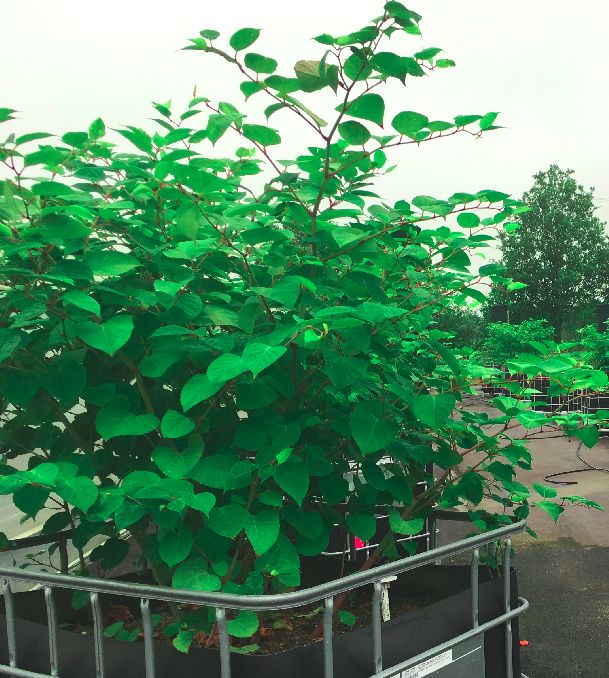
\includegraphics[width=0.65\linewidth]{renouee_aerien3}}
\end{figure}
\end{minipage}
\begin{minipage}{0.45\linewidth}
%\bigbreak \bigbreak
Rhizome
\begin{figure}[H] 
%\center{\includegraphics[width=0.75\linewidth]{renouee_rhizome}}
\center{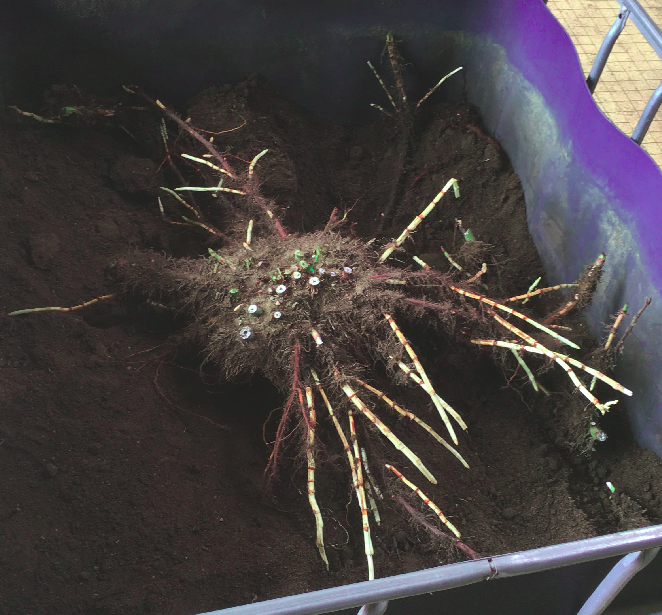
\includegraphics[width=0.80\linewidth]{renouee_rhizome3.png}}
%\caption{Extrait de \cite{smith2007simulation}} 
\end{figure}
\end{minipage}

\bigbreak

Stem: from 1 to 3 meters.

\smallbreak
Rhizome: up to 8 cm diameter, length : 15 - 20 m, depth: 2 - 3 m, represents 2/3 of the total biomass of the plant.

\smallbreak
The rhizome withstands the cold and enables to spend the bad season burried in the ground.
\end{frame}





\begin{frame}{Clonal development of the Japanese knotweed.}

\begin{figure}[H] 
\center{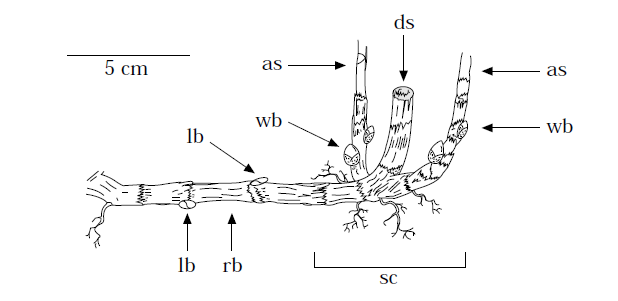
\includegraphics[width=0.7\linewidth]{adachi_rhizome_bud2}}
\caption{Diagram of the development of stems and buds along the rhizome, extracted from\cite{adachi1996central} 
as: current aerial shoot, ds: dead aerial shoot, rb: rhizome, sc: shoot clump, lb: lateral bud, wb: winter bud.}
\label{network_renouee_3}
\end{figure}

\textbf{References:} \cite{adachi1996central}, \cite{dauer2013elucidating}, \cite{price2002seasonal}, \cite{beerling1994fallopia}, \cite{de2001viability}.

\end{frame}







%%%%%%%%%%%%%%%%%%%%%%%%%%%%%%%%%%%%%%%%%%%%
\subsection*{Litterature on modeling the Japaneee knotweed evolution}
\begin{frame}{Litterature on modeling the Japaneee knotweed evolution}

\begin{itemize}
\noindent
\begin{minipage}{0.60\linewidth}
\item  
\cite{smith2007simulation} have constructed a 3D correlated random walk for the development of the underground rhizome network.
\end{minipage}
\begin{minipage}{0.35\linewidth}
\begin{figure}[H] 
\center{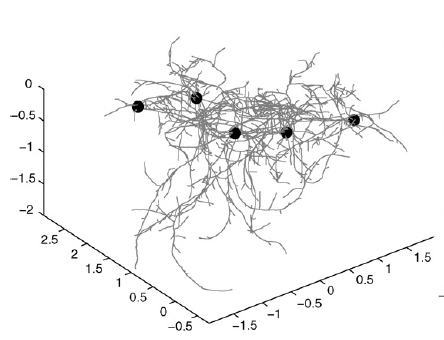
\includegraphics[width=1\linewidth]{network_renouee_5}}
\end{figure}
\end{minipage}

\item
\cite{dauer2013elucidating} propose an "Integral Projection Model" (IPM), inspired by the "Matrix Population Model", for the dynamics of the plant at the level of a stand.

\bigbreak
\item 
\cite{gourley2016mathematical} have developed a model of biocontrol of the knotweed, based on the insect Psyllid Aphalara Itadori, which feeds on the sap of the stems of the knotweed. Deterministic model that describes the evolution of the number of insects (larvae and adults) as well as the evolution of the total biomass of stems and rhizome.
\end{itemize}

\end{frame}




%%%%%%%%%%%%%%%%%%%%%%%%%%%%%%%%%%%%%%%%%%%%%%
\section*{The model we propose}
\subsection*{Frame and objective of the model}
\begin{frame}{Dynamical model for the knotweed}
\textbf{Objective:} Describe the dynamics of Japanese knotweed at the local scale and the effects of mowing on it.

\smallbreak
The mathematical formalism is the one of the \textbf{measure-valued stochastic processes}.

\smallbreak
The model presented in this section is inspired by the work of \cite{fournier2004microscopic} and \cite{tran2006modeles}.

\smallbreak
 The individuals, here the crowns 
 %\textcolor{red}{demander à Fanny si c'est bien ce terme, ou shoot clump} 
 (i.e. the places where the terminal buds are located and from which the stems sprout) are characterized by:
 \begin{itemize}
\item  their position (in the plan)
 \item  a trait describing the underground biomass (i.e. that of the rhizome that is connected to the crown).
\end{itemize}
 
\end{frame}






%\begin{frame}{Notations}
%We introduce the following notations 
%\begin{itemize}
% \item $ \chi = \R^2 \times \R_+$. 
% \item $\Mcal_F ( \chi )$  [resp. $\Pcal(\chi)$] the set of finite measure (resp. probability measure) on $X$. 
%\item   $\Mcal \subset \Mcal_F ( \chi)$: finite point measures whose point mass is 1 or 0.  
%\begin{equation*}
%\Mcal = \left\{  \sum_{i=1}^n  \delta_{x_i,a_i} ~ , n \geq 0 , ~ (x_1,a_1), \ldots, (x_n,a_n) \in      \chi  \right\}
%\end{equation*}   
%\end{itemize}
%
%In the model, a crown is represented by a Dirac mass $\delta_{(x,a)}$, with $(x,a) \in \chi$.
%
%\smallbreak
%The set of all crowns at time $t$ is described by the measure $Z_t \in \Mcal$.
%\end{frame}




\subsection*{The phenomena taken into account}

\begin{frame}{Events occurring in the model}

At each time, we calculate the next time at which there is an event. There are three possible events: 
\bigskip 
\begin{itemize}
\item a birth of a new crown: birth rate depending on positions, law for the dispersal distance and intra-specific competition zone
%\bigbreak
\item a death of a crown: mortality rate depending on biomass
%\bigbreak
\item the mowing of a proportion $proportionMowing$ of individuals in the population. The effect of mowing is a decreasing function of the the biomass.

\bigskip 
\item Between those events, the biomass of each crown evolves in a deterministic way.
\end{itemize}
\end{frame}






\subsubsection{Birth and dispersal of the created individual}

%\begin{frame}{Birth and dispersal of the created individual}
%
%\bigbreak
%\begin{minipage}{0.55\linewidth}
%An individual with trait $(x,a)$ produces an individual in $x'$ at rate $b(x,Z)$.
%We choose a Gamma law with parameters $(shape,scale)$ for the law of the dispersal distance of the daughter crown.
%\end{minipage}
%\begin{minipage}{0.35\linewidth}
%\begin{figure}[H] 
%\center{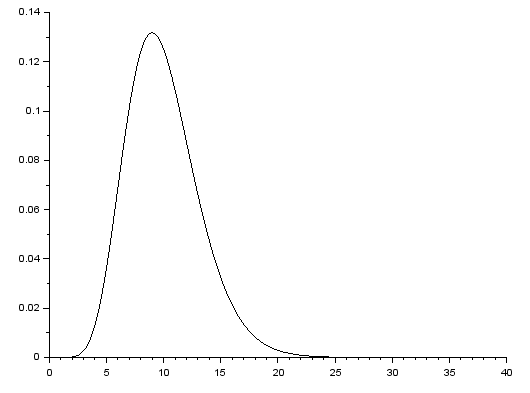
\includegraphics[width=1\linewidth]{fonction_dispersion}}
%\end{figure}
%\end{minipage}
%
%\end{frame}



\begin{frame}{Birth and dispersal of the created individual}
Birth rate  depends on the neighbouring individuals present at a distance smaller than $distanceParent$. That allows us to account for the effects of apical dominance.

\bigbreak
\begin{minipage}{0.55\linewidth}
%An individual with trait $(x,a)$ produces an individual in $x'$ at rate $b(x,Z)$.
We choose a Gamma law with parameters $(shape,scale)$ for the law of the dispersal distance of the daughter crown. %The parameters ($shape$, $scale$) of the distribution will be subject to calibration.
\end{minipage}
\begin{minipage}{0.35\linewidth}
\begin{figure}[H] 
\center{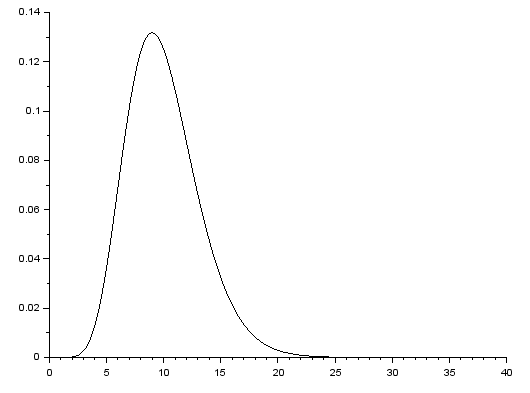
\includegraphics[width=1\linewidth]{fonction_dispersion}}
\end{figure}
\end{minipage}

%Model the phenomenon of intra-specific competition by considering that an individual is really born only if it does not fall too close to an already existing crown
\bigbreak
The new born individual must therefore be at a distance larger than $distanceCompetition$ from its neighbours not to fall in the zone of intraspecific competition.


\end{frame}






%\begin{frame}{Mortality}
%
%\begin{itemize}
%\item Hypothesis: the mortality rate is independent of the position $x$ of an individual. \bigbreak
%\item An individual living at time $t$ with a biomass $a(t)$ dies at the rate $m(a(t))$.
%\bigbreak
%\item The mortality $m$ is \textbf{a decreasing function of the biomass}: an individual with a low biomass, either because it has just been created or because it has undergone mowing, will have a higher rate of mortality.% ie taux de mortalité aux individus ayant un trait de biomasse faible.
%\end{itemize}
%\end{frame}




\subsubsection*{Evolution of the biomass:}
%
%\begin{frame}{Evolution of the biomass}
%
%The rhizome biomass associated with a crown evolves (in the absence of a mowing or mortality event) according to the following equation:
%\begin{equation}
%\label{VonBert}
%\frac{da(t)}{dt}= L  ( K - a(t) ) 
%\end{equation}
%
%where $L$ is the low biomass growth rate and $K$ is the asymptotic biomass.
%
%\bigbreak 
%
%We are able to solve explicitly Equation \eqref{VonBert}.
%
%We denote by $A_b$ the flow: $ t \rightarrow A_b(t,t_0,a_0)$ associated with the ordinary differential equation \eqref{VonBert}.
%\end{frame}



%%%%%%%%%%%%%%%%%%%%%%%%%%%%%%%%%%%%%


\begin{frame}{Mowing}
Effects of mowing on rhizome development are poorly known.
\begin{itemize}
\item Hypothesis: reduction of underground biomass, rhizome resources used for growth of aerial parts \cite{gerber2010evaluating}, \cite{rouifed2011contrasting}
\item No influence of the distribution of the mowing dates, only the mowing number matters \cite{seiger1997mechanical}
\item Modeling choice: after a mowing, the underground biomass is directly impacted and becomes $a.F (a)$, where $F(a) \in [0,1]$. It is assumed that the effect of mowing is more important for low biomasses $ \Rightarrow F$ \textbf{increasing}.
\end{itemize}

\begin{equation*}
\forall a \in \R_+, ~F(a) = 1- exp(-mowingParameter  * a)
\end{equation*} 

\end{frame}




\begin{frame}{Random mowing technique}
\begin{figure}[H] 
\center{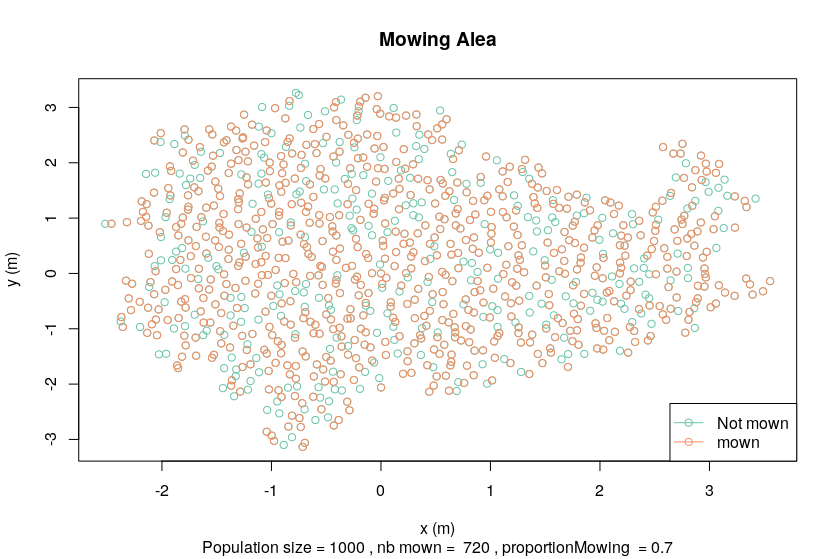
\includegraphics[width=0.70\linewidth]{"comparaison mowing technique"/Alea4}}
\caption{Represents the crowns that would be mown during a mowing event with the Random technique. A proportion of mown plants is imposed. The coordinates are in meters.}
\label{MTAlea}
\end{figure}
\end{frame}





\begin{frame}{Side mowing technique}
\begin{figure}[H]
\center{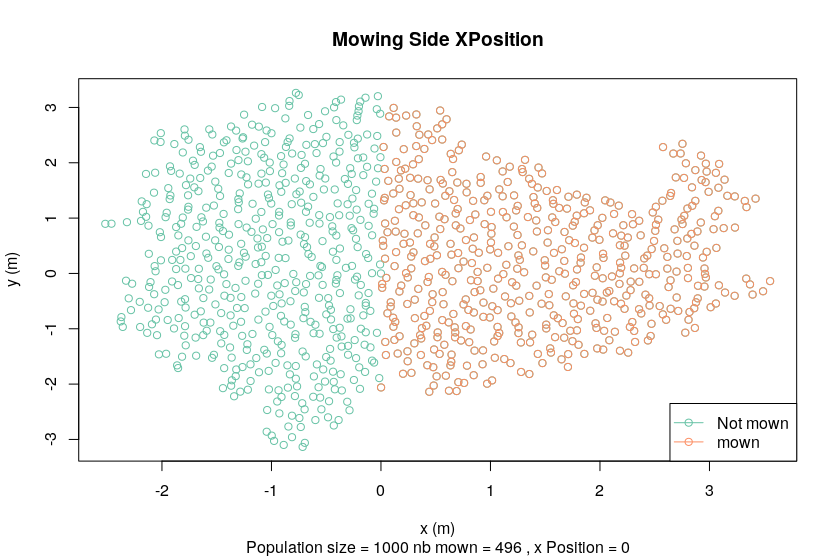
\includegraphics[width=0.60\linewidth]{"comparaison mowing technique"/SideXPosition4}}
\caption{Represents the crowns that would be mown when imposing a \emph{position} at the right of which all plants are mown.} 
\label{MTSideXPosition}
\end{figure}
% Throughout the rest of the presentation, it is the RANDOM technique that is used.
\end{frame}



%%%%%%%%%%%%%%%%%%%%%%%%%%%%%%%%%%


%\subsection{Les Paramètres du modèle}
\begin{frame}{Model Parameters}
  \scriptsize
    
\begin{tabular}{lll}
	\hline
   Variable & Description                            \\ %  & valeur \\
   	\hline
   Biomass  &                              \\ % &  \\
   	\hline
    $K$       &  maximal biomass   (g)    \\ % & 5  \\
    $L$      &  growing rate for low biomasses \\ %, & 0.3  \\
    $a_0$      &  initial  biomass of a born crown (g)  \\ % & 0.5   \\
       	\hline
   Mowing &                         \\ %      & 	 \\
		\hline   
  %  $\tau$      & mean number of mowing events a year \\ 
  %  $proportionMowing$      &  proportion of mown plants \\ 
    $mowingParameter$  &  effect of mowing \\  
          \hline
   Mortality &                         \\ 
		\hline
    $deathParameterScaling$  & for the small biomasses \\ % & 1.5  \\ 
     $deathParameterDecrease$  &  decrease speed of the mortality rate\\ %& 1  \\
       \hline
  Birth &                           \\ %    &  \\
		\hline
  $distanceParent$      &  distance of apical dominance (m) \\ % & 0.15m \\
    $distanceCompetition$       &   intra spécific competition distance (m) \\ % & 0.15m  \\
 	$\bar{b}$    &  birth rate (ideal conditions) \\ %& 1 \\
    $ (\text{shape},\text{scale})$     &   Gamma law, dispersion of the created individual\\ %& (10,1)
     \hline
\end{tabular}
 %\captionof{table}{Tableau récapitulatif des paramètres du modèle pour les simulations}
 %\label{tableau_recap_param}
 
\bigbreak

Management parameters:
\begin{itemize}
\item initial population size: $ InitialPopSize $
\item mean number of mowing events a year: $\tau$
\item management project duration: $T$ 
\item proportion of mown crowns: $proportionMowing$
\end{itemize}

\end{frame}




%%%%%%%%%%%%%%%%%%%%%%%%%%%%%%%%%%%%%%%%%%%


%\subsection*{Stochastic Differential Equation}
%\begin{frame}{Stochastic Differential Equation}
%\begin{align*}
%\label{equation_sto} 
% Z_t & =  \sum_{i=1}^{N_0} \delta_{( X_i(Z_0) , A_b(t,0,A_i(Z_0) )} \\
% & +  \int_0^t \int_{\N^*} \int_{\R_+} \int_{\R^2}  1_{ \{  i \leq  N_{s-}  \} } \delta _{( X_i(Z_s)+z , A_b(t,s, a_0 ) ) } \\ 
%& \times   1_{ \{  \theta \leq b(X_i(Z_s), Z_s ) \} }   1_{ \{ X_i(Z_s) + z ~ \in ~ C_{X_i(Z_s),Z_s} \} } \times M_1(ds,di,d\theta,dz) \\ 
%& +  \int_0^t \int_{[0,1]^{N^*}}  ~ \sum_{i=1}^{N_{s^-}}  1_{ y_i \leq proportionMowing } ~\\
%&( \delta_{( X_i(Z_s) , A_b(t,s,A_i(Z_{s^-}).F(A_i(Z_{s^-}) ) ))} -  \delta_{( X_i(Z_s) , A_b(t,s,A_i(Z_s)) )} )   M_2(ds,dy)  \\
%&- \int_0^t \int_{\N^*} \int_{\R_+}  1_{ \{  i \leq  N_{s-}   \} }   1_{ \{  \theta \leq m( A_i(Z_s) ) \} }  \delta _{( X_i(Z_s) , A_b(t,s,A_i(Z_s) ) } M_3(ds,di,d\theta). 
%\end{align*}
%
%\small{$M_1(ds,di,d\theta,dz)$ is a Poisson point measure on $E_1:= \R_+ \times \N^* \times \R_+ \times  \R^2 $  with intensity $ \nu_1 = ds \otimes n(di)  \otimes d\theta \otimes  D(dz) $. }
%\end{frame}




\section*{Large population limit}

\begin{frame}{Large population limit}


Under boundary conditions over the birth and death rates, the stochastic differential equation admits a unique pathwise strong solution (and an upper bound to the growth of the population). 
%$(Z_t)_{t \in \R_+} \in \D( \R_+ , \Mcal( \chi ) )$ such that for all  $T>0$, the number of individuals at time $t \leq T,N_t :=  \langle Z_t,1 \rangle = \int_{\R^2 \times \R} Z_t(dx,da) $ satisfies :
%\[  \E[ \sup_{t \in [0, T]} N_t ] < \E [ N_0] e^{\bar{b}T} < \infty .   \]
%This gives in particular an upper bound to the growth of the population when there is no management


\bigbreak

\textbf{Objective:} Study of a renormalisation of the Stochastic Differential Equation solution $(Z^n)_{n \in \N}$ associated with the dynamics. 

\begin{itemize}
\item Simplification of the SDE: withdrawal the mowing term.

\item Initial population size of order $n$, no modification of the interaction between individuals. 
\end{itemize}

\smallbreak
\textbf{Result:} law convergence of the sequence of renormalised processes toward a process solution of an integro-differential equation :

%\begin{flalign*}
% \langle \xi_t , f_t \rangle =  \langle \xi_0 , f_0 \rangle  +  
%\int_0^t  \int_{\chi} \big[  v(a) \nabla_a f_s (x,a) + \frac{df_s}{ds}(x,a)  \\
%  +\int_{\R^2} f_s(x+z,a_0)b(x,\xi_s ).h(x,z,\xi_s )d(dz)  -   f_s(x,a)  m(a) ) \big]  \xi_s (dx,da) ds. &&
%\end{flalign*}

% Ainsi, en grande population, on pourra remplacer l'étude de l'équation différentielle stochastique par l'étude de cette nouvelle équation. 

\smallbreak
The techniques used for this result are those developed in \cite{tran2006modeles}.



\end{frame}



%%%%%%%%%%%%%%%%%%%%%%%%%%%%%%%%%%%%%%%%%%%%%%
%\section{Calibration du modèle}
%\subsection{les données, la méthode}
%\begin{frame}{Calibration du modèle :les données, la méthode}
%
%\end{frame}
%
%%%%%%%%%%%%%%%%%%%%%%%%%%%%%%%%%%%%%%%%%%%%%
%\subsection{Les résultats de la calibration}
%\begin{frame}{Les résultats de la calibration}
%
%\end{frame}
%



\section*{Calibration: Proposition of a set of parameters for the dynamics of evolution of the plant}\label{Calibration}
\subsection*{F.Martin data used to compare model outputs}  \label{Data_Matin}

\begin{frame}{}
\center \huge
ANALYSIS OF THE MODEL BY SIMULATIONS
%\huge 
 \bigbreak \bigbreak
CALIBRATION
\end{frame}



%%%%%%%%%%%%%%%%%%%%%%%%%%%%%%%%%%%%%%%%%%%%

\begin{frame}{Reminder of model parameters}
  \scriptsize
    
\begin{tabular}{lll}
	\hline
   Variable & Description                            \\ %  & valeur \\
   	\hline
   Biomass  &                              \\ % &  \\
   	\hline
    $K$       &  maximal biomass   (g)    \\ % & 5  \\
    $L$      &  growing rate for low biomasses \\ %, & 0.3  \\
    $a_0$      &  initial  biomass of a born crown (g)  \\ % & 0.5   \\
       	\hline
   Mowing &                         \\ %      & 	 \\
		\hline   
  %  $\tau$      & mean number of mowing events a year \\ 
  %  $proportionMowing$      &  proportion of mown plants \\ 
    $mowingParameter$  &  effect of mowing \\  
          \hline
   Mortality &                         \\ 
		\hline
    $deathParameterScaling$  & for the small biomasses \\ % & 1.5  \\ 
     $deathParameterDecrease$  &  decrease speed of the mortality rate\\ %& 1  \\
       \hline
  Birth &                           \\ %    &  \\
		\hline
  $distanceParent$      &  distance of apical dominance (m) \\ % & 0.15m \\
    $distanceCompetition$       &   intra spécific competition distance (m) \\ % & 0.15m  \\
 	$\bar{b}$    &  birth rate (ideal conditions) \\ %& 1 \\
    $ (\text{shape},\text{scale})$     &   Gamma law, dispersion of the created individual\\ %& (10,1)
     \hline
\end{tabular}
 %\captionof{table}{Tableau récapitulatif des paramètres du modèle pour les simulations}
 %\label{tableau_recap_param}
 
\bigbreak

Management parameters:
\begin{itemize}
\item initial population size: $ InitialPopSize $
\item mean number of mowing events a year: $\tau$
\item management project duration: $T$ 
\item proportion of mown crowns: $proportionMowing$
\end{itemize}

\end{frame}


%%%%%%%%%%%%%%%%%%%%%%%%%%%%%%%%%%%%%%%%%%%%

\begin{frame}{F.Martin data}

\bigbreak 

\noindent
\begin{minipage}{0.45\linewidth}
\begin{figure}[H] 
\center{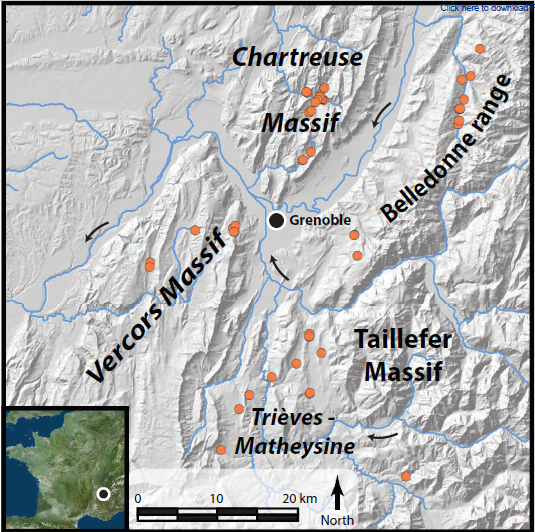
\includegraphics[width=0.97\linewidth]{renouee_alpes_Martin}}
\caption{Extrait de \cite{FMartin17}.}
\end{figure}
\end{minipage}
\begin{minipage}{0.45\linewidth}

48 stands of knotweeds in the French Alps (various altitudes). 
\smallbreak
Measurements carried out in 2008 and in 2015: on the stands themselves (outline, number of stems, ...) and on biotic and abiotic variables.
%( factuers biotiques : ensemble des intéractions du vivant sur le vivant au sein d'un écosystème : ressources alimentaires,...)
 %(action du non vivant sur le vivant : structure du sol, teneur en minéraux, climatique, température, lumière, chimique, topographique (altitude)).

%The study was conducted on 48 stands located in four mountain ranges (Belledonne,  Chartreuse, Trièves- Matheysine, and Vercors) of the French Northern Alps

\bigbreak
Variability in observed stands: size (less than $1m^2$ to $350 m^2$), area (proximity of watercourse, road, forest, abandoned land)

\end{minipage}
\end{frame}



%%%%%%%%%%%%%%%%%%%%%%%%%%%%%%%%%%%%%%%%%%%%

\begin{frame}{F. Martin data- Calibration}
\begin{itemize}
\item In model outputs, we have the final and initial population areas and sizes.
\item In F. Martin's article, we use data on areas and densities of stands (so we have access to the size of the population) in 2008 and 2015.
\end{itemize}

\bigbreak

	 \footnotesize
\begin{tabular}{lllllll}
	\hline
   stand   &   size 2008   & area 2008   &   size2015  & area 2015  & $\tau$ & FullMow  \\  
   	\hline
    1 &  261  &  14.525     &  112   &      10.815    &  0   &   0   \\
    2 & 1878  &  52.177     &   872  &			42.187  &  1   &   0   \\
    3 & 1063  &  75.899 	 &  1493   &	  72.829    &  1 	&  1   \\
    4 & 1771  &  104.203    &  852   &      49.273    &  2   &  1   \\
 $\vdots$ &   $\vdots$ & $\vdots$ &  $\vdots$ &  $\vdots$  &   $\vdots$ &  $\vdots$ \\    
     \hline
\end{tabular}
\end{frame}


%%%%%%%%%%%%%%%%%%%%%%%%%%%%%%%%%%%%%%%%%%%%

\begin{frame}{Method for the calibration}
The OpenMOLE software proposes a method derived from genetic algorithms for the calibration of models.

\bigbreak
The algorithm explores the parameter space to find the minimal distance between the observations and the simulations (the algorithm manages the stochasticity of the model).
\bigbreak

As distance between simulations and observations, we take for each stand and each type (area or size) the distance: $ \frac{ | simu - data |}{ data}$.

\begin{figure}[H] 
\center{
\includegraphics[width=0.30\linewidth]{openMOLE}}
%\caption{A Computational Engine for Custom Simulation Experiments}
\end{figure}

\textbf{Reference :} \cite{Reuillon2013}
\end{frame}



%%%%%%%%%%%%%%%%%%%%%%%%%%%%%%%%%%%%%%%%%%%%
\subsection*{The result of the calibration}

\begin{frame}{The result of the calibration}
\
\begin{tabular}{lr}
	\hline
     Variable			    &   Valeur Calibration    \\  
   	\hline
		K						&	12.72	\\	
		L						&	0.26	\\	
		distanceCompetition		&	0.15	\\	
		distanceParent			&	0.20	\\	
		shape					&	4.34	\\	
		scale					&	2.36	\\	
		deathParameterDecrease	&	2.32	\\	
		deathParameterScaling	&	1.12	\\	
		mowingParameter			&	0.11	\\	
		bbar					&	0.18	\\	
		a0						&	1.73	\\	
		delta					&	26.06	\\	
		evolution.samples		&	79		\\	
     \hline                                   
\end{tabular}

\end{frame}

%%%%%%%%%%%%%%%%%%%%%%%%%%%%%%%%%%%%%%%%%%%%  x
\subsection*{Reasons for satisfaction.}

\begin{frame}{\large{Agreement between calibrated values and experts' statements}}

\begin{itemize}
\item \footnotesize{The parameters $distanceCompetition$ and $distanceParent$, close to experts' statements.}
\smallbreak
\begin{tabular}{lll}
	\hline
     Variable			    &   Calibration value     &   experts' statements \\
   	\hline
		distanceCompetition		&	0.15		&		$\approx$ 0.15	\\
		distanceParent			&	0.20		&		$\approx$ 0.15	\\
     \hline                                   
\end{tabular}

\bigbreak %\footnotesize
\item \footnotesize{The law for the dispersal of individuals $\Gamma(shape=4.34, scale=2.36)$, in compliance with experts' statements.}

\begin{figure}[H] 
\center{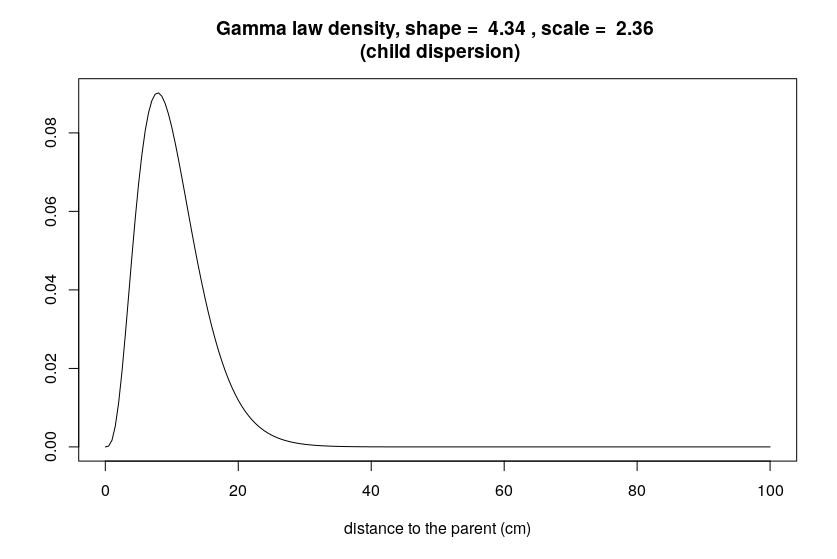
\includegraphics[width=0.60\linewidth]{fonctionsModeleParamMin/loigammaParamMin}}
% \caption{Gamma law for the dispersal distance of a child, with law parameters from calibration.}
\label{loigammaCalibration}
\end{figure}

\end{itemize}

\end{frame}




%%%%%%%%%%%%%%%%%%%%%%%%%%%%%%%%%%%%%%%%%%%%
\begin{frame}{\large{Agreement between calibrated values and experts' statements}}
\begin{itemize}

\item  \footnotesize{The ratio of the values of K (maximum biomass), and $a_0$ the biomass of the individuals at birth, which is 7.5 (a ratio of about 10 is expected).}

\bigbreak

\begin{tabular}{llll}
	\hline
     \scriptsize{Variable} &   \scriptsize{Calibration value}  & \scriptsize{Calibration values ratio} & \scriptsize{Experts' statements ratio} \\
   	\hline
		K			&	12.72		& \multirow{2}{*}{7.5} &  \multirow{2}{*}{$\approx$ 10}		\\
		$a_0$			&	1.73		&							&							  \\
     \hline                                   
\end{tabular}

\bigbreak
\item  \footnotesize   Mortality rate:
\begin{figure}[H] 
\center{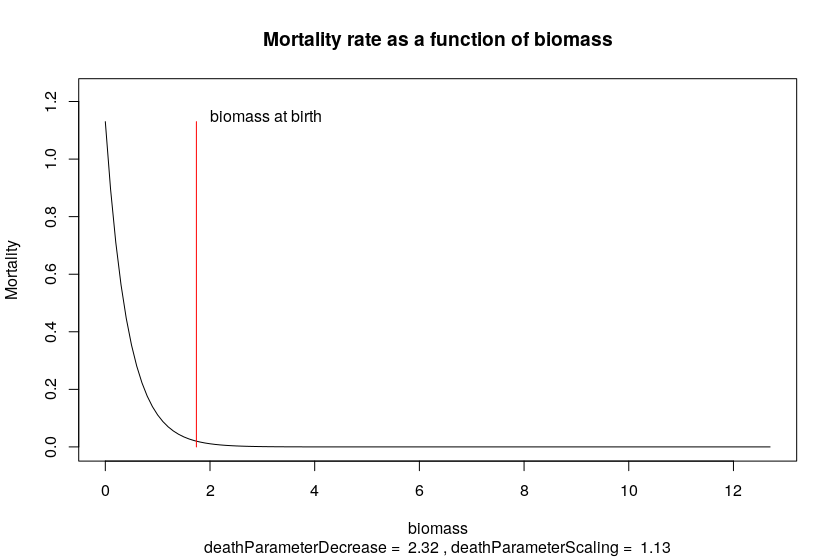
\includegraphics[width=0.50\linewidth]{fonctionsModeleParamMin/MortalityParamMin}}
\caption{ \scriptsize{Mortality rate of a crown according to its biomass. We note that a crown that is not mown keeps a very low mortality rate, which agrees with field observations.}}
\label{MortalityParamMin}
\end{figure}

\end{itemize}
\end{frame}





%%%%%%%%%%%%%%%%%%%%%%%%%%%%%%%%%%%%%%%%%%%%

\begin{frame}{}
\center \huge
ANALYSIS OF THE MODEL BY SIMULATIONS
%\huge 
 \bigbreak \bigbreak
INFLUENCE OF MOWING PARAMETERS
\end{frame}




\section*{Law of the outputs}
\begin{frame}{Law of the outputs, replications}
\begin{figure}[H] 
\center{\includegraphics[width=0.7\linewidth]{"loi sortie"/"FDR sans extinction"/"FDR aire finale sans extinction"}}
\caption{\footnotesize Probability Distribution Function of the final area, obtained with an initial population size = 1500, $\tau = 4$,  $proportionMowing = 0.9$, and $T=8$.}
\end{figure}
\end{frame}





%%%%%%%%%%%%%%%%%%%%%%%%%%%%%%%%%%%%%%%%%%%%
\begin{frame}{Comparison of initial and final area densities.}
\begin{figure}[H] 
\center{\includegraphics[width=0.6\linewidth]{"loi sortie"/"comparaison aire ini aire finale"/"comparaison densite aire initiale finale"}}
\caption{\footnotesize Density of the Gaussian laws of the initial and final areas, obtained from the empirical averages and variances. Initial population size = 1500, $\tau = 4$,  $proportionMowing = 0.9$, and $T=8$.}
\end{figure}
\end{frame}






\begin{frame}{Influence of $T$ on the final average area}
\begin{minipage}{0.75\linewidth}
\small{We plot the regression curves obtained for different $\tau$. [InitialPopSize = 1500 and $proportionMowing = 0.9$ fixed].}
\begin{figure}[H] 
\center{\includegraphics[width=0.82\linewidth]{"loi sortie"/"influence de T"/"courbes de aire moyenne vs T differents tau"}}
\caption{\footnotesize Quadratic regression curves  of the mean final area as a function of $T$, for different $\tau$.}
\end{figure}
\end{minipage}
\begin{minipage}{0.20\linewidth}
\bigbreak \bigbreak 
\begin{figure}[H] 
\center{\includegraphics[width=0.9\linewidth]{"loi sortie"/"influence de T"/"Graph sans titre 3"}}
\caption{\footnotesize Cross section.}
\end{figure}
\end{minipage}
\end{frame}




%%%%%%%%%%%%%%%%%%%%%%%%%%%%%%%%%%%%%%%%%%%%
\section*{Summary}

\begin{frame}{
Summary of the influences of the management parameters on the average values of the outputs
}

%\bigbreak

%\scriptsize
\renewcommand{\arraystretch}{1.8}
\begin{tabular}{|l|l|l|l|}
	\hline
   Initial / Final   &   Param   			&  Average Area   & Average Size   \\  
   	\hline
    Initial  &    InitialPopSize		&     linear $\nearrow$      &     linear$\nearrow$    \\
	\hline	    
    Final &   InitialPopSize	& linear   $\nearrow$  &   linear $\nearrow$\\
	\hline	        
	 \multirow{2}{*}{Final} &  \multirow{2}{*}{T}  &  linear$\nearrow$ ($\tau$ weak)   & linear $\nearrow$  \\
 \cline{3-4} 
	& &  quadratic  $\searrow$	 ($\tau$ high) & exponential $\searrow$ \\
	\hline    
    Final &   $\tau$ 	weak &    linear $\nearrow$ or $\searrow$	&  linear $\searrow$  \\
    Final &   $\tau$ 	high   &   linear $\searrow$	&  exponential  $\searrow$  \\
     \hline
     
\end{tabular}

%\bigbreak
%\pause
%Formulas for the  final size and area, for $\tau \gtrsim 2$:
% \[  Final ~  Size ~ = Initial ~ Size \times exp(- T  .( \tau - a)/b ), \] with $a,b \in \R$ constants.
%
%\[ Final ~  Area ~ = \max( c \times tau \times t^2 + 0.04 \times Initial ~ Size , 0)  \text{, with } c \in \R \text{ constant}.  \]
\end{frame}


\begin{frame}{Formulas for the  final size and area}
Wa have the more general result:
\begin{Resu}
For $\tau \gtrsim 2$:
\[  Final ~  Size ~ = Initial ~ Size \times exp(- T  .( \tau - a)/b ), \] with $a,b \in \R$ constants,

\bigbreak 
and,
\[ Final ~  Area ~ = \max( c \times tau \times t^2 + 0.04 \times Initial ~ Size , 0)\]  with $c \in \R$ constant. 

\end{Resu} 


\end{frame}



\begin{frame}{Important remark for the formulas}
\footnotesize
Formulas obtained for the mean output quantities are still relevant for direct outputs. 

\begin{figure}[h]
    \centering
     \includegraphics[ width=0.60\linewidth]{"size vs T global2"}  %[width=5cm,height=5cm]
     \caption{\footnotesize Black circles represent stand sizes resulting of 50 replications with $\tau = 4$, initial population size = 1000, and varying $T$.
The red line is the function of $T$ defined by Equation for the mean final size. It has been found with a regression on a far bigger set of points than the subset selected to plot this example. }
\end{figure}
\end{frame}











%%%%%%%%%%%%%%%%%%%%%%%%%%%%%%%%%%%%%%%%%%%%
\section*{Perspectives}
\begin{frame}{Perspectives}

%\textcolor{blue}{Regarding the presented study:} 
%\begin{itemize}
%\item Establish the limit in large population with mowing term.
%\end{itemize}

\bigbreak
\textcolor{primaryGreenOM}{Take an interest in two other questions managers face:} 
\begin{itemize}
\item At the scale of a landscape with several knotweed stands, how to distribute the mowing effort (intensity / frequency) between the different stands?

$\rightarrow$  Modeling the dispersion due to mowing.

\item Compare mechanical engineering (mowing) vs ecological engineering (willow)? 

$\rightarrow$  Model the influence of the shadow on the dynamics of knotweed.
\end{itemize}

\bigbreak
\textcolor{primaryGreenOM}{Pose viability problems in stochastic formalism.}
\end{frame}





\begin{frame}{OpenMOLE USER CASE} %References

\textcolor{primaryGreenOM}{OpenMOLE USER CASE}, joint work with G.Chérel
\smallbreak
On Gitlab:
\smallbreak
\url{https://gitlab.iscpif.fr/gcherel/renouee/blob/master/README_en.html}

\bigbreak

and on \textcolor{primaryGreenOM}{OpenMOLE blog}:
\smallbreak
\url{https://blog.openmole.org/}


\bigbreak

More details can be found in:

%Lavallée, F., Smadi, C., Alvarez, I., Reineking, B., Martin, F.-M., Dommanget, F., and Martin, S.
\cite{lavalleeQuelsApportsModelisation}
%Lavallée \& al. 
Quels apports de la modélisation pour l’aide à la gestion de la renouée du Japon. \textit{Sciences Eaux et Territoires}.

\smallbreak
\cite{lavalleeAStochasticIndividual}
%Lavallée \& al. 
A stochastic individual based model for the growth of a stand of japanese knotweed including mowing as a management technique. \textit{Submitted to Ecological Modelling}, \url{https://arxiv.org/abs/1902.06971}



\end{frame}



\section{Thanks for your attention!}
%\begin{frame}
%\center \huge Thanks for your attention!
%\end{frame}







%%%%%%%%%%%%%%%%%%%%%%%%%%%%%%%%%%%%%%%%%%%%
\section*{annexe après la fin de la présentation}

\makeatletter
\setbeamertemplate{footline}
{
  \leavevmode%
  \hbox{%
  \begin{beamercolorbox}[wd=.333333\paperwidth,ht=2.25ex,dp=1ex,center]{author in head/foot}%
    \usebeamerfont{author in head/foot}\beamer@shortauthor
  \end{beamercolorbox}%
  \begin{beamercolorbox}[wd=.333333\paperwidth,ht=2.25ex,dp=1ex,center]{title in head/foot}%
   % \usebeamerfont{title in head/foot}\insertsubsection ou \insertsection
%%%%%%%%%%%%%% pour mettre la section à la place du titre
	\usebeamerfont{title in head/foot}\beamer@shorttitle
  \end{beamercolorbox}%
  \begin{beamercolorbox}[wd=.333333\paperwidth,ht=2.25ex,dp=1ex,center]{date in head/foot}%
    \usebeamerfont{date in head/foot}\insertshortdate{}%\hspace*{6em}
    %\insertframenumber{} / \inserttotalframenumber\hspace*{2ex} 
  \end{beamercolorbox}}%
  \vskip0pt%
}
\makeatother 

	
\backupbegin


%%%%%%%%%%%%%%%%%%%%%%%%%%%%%%%%%%%%%%%
%  Faire varier Tau
%%%%%%%%%%%%%%%%%%%%%%%%%%%%%%%%%%%%

\begin{frame}{Varying the mean number of mowing events}
\textbf{Question :} We vary the mean number of mowing events each year. Which management strategy minimizes the final area?

\bigbreak 
We set the total number of mowing events over the all period of management equal to  $N_{tot}$, and total number of mowing events over a year equal to  $\tau_{max}$.
The aim is to find $( \tau_1, \ldots , \tau_T)$ which minimizes the final area.

\bigbreak 
The set of admissible configurations is defined by
\[ X := \{ ( \tau_1, \ldots , \tau_T) \in [ 0 ; \tau_{max}]^T  | \sum_{i=1}^{T} \tau_i = N_{tot} \} \]

\end{frame}



\begin{frame}%[fragile]
\frametitle{Varying the mean number of mowing events}

\smallbreak
Example: $T=4$, $N_{tot} = 5 \times 4$, $\tau_{max} = 15 $,  $(5,5,5,5) \in X$, $(8,6,4,2) \in X$.  $ \#(X) = 1631$.

\bigbreak 
Practical issue: Using reasonable size of configuration set, we can perform a \textit{sample} (DirectSampling and filter), and deal with stochasticity by hand.

\pause
\smallbreak  %\bigbreak
But this is not achievable for large configuration sets.
\smallbreak
Example: $T=8$, $N_{tot} = 5 \times 8$. %, $(5,5,5,5,5,5,5,5) \in X$, $(8,6,4,2,8,6,4,2) \in X$.  $ \#(X) = 1631$
%java.lang.OutOfMemoryError: Java heap space
%other solution, not exactly the same pb: more general, do not impose the sum of tau to be equal to Ntot.
\smallbreak
\pause
More general situation: $N_{tot}$ varies. %, just consider $\tau_{max}$.

Then we use NSGA2 algorithms, which deals with stochasticity, considering real numbers as inputs parameters, with 2 objectives: minimizing the invaded area at time $T$ and the total number of mowing events $\sum_{i=1}^{T} \tau_i$. We obtain a Pareto front.  
%$\tau_i \in [0;\tau_{max} $, to impose the condition $\sum_{i=1}^{T} \tau_i = N_{tot}$ we can impose an other objective to minimize :  $\sum_{i=1}^{T} \tau_i - N_{tot} $  
  
\end{frame}



%%%%%%%%%%%%%%%%%%%%%%%%%%%%%%%%%%%%%%%
%  Mechanism + math formalism
%%%%%%%%%%%%%%%%%%%%%%%%%%%%%%%%%%%%

\begin{frame}{Notations}
We introduce the following notations 
\begin{itemize}
 \item $ \chi = \R^2 \times \R_+$. 
 \item $\Mcal_F ( \chi )$  [resp. $\Pcal(\chi)$] the set of finite measure (resp. probability measure) on $X$. 
\item   $\Mcal \subset \Mcal_F ( \chi)$: finite point measures whose point mass is 1 or 0.  
\begin{equation*}
\Mcal = \left\{  \sum_{i=1}^n  \delta_{x_i,a_i} ~ , n \geq 0 , ~ (x_1,a_1), \ldots, (x_n,a_n) \in      \chi  \right\}
\end{equation*}   
\end{itemize}

In the model, a crown is represented by a Dirac mass $\delta_{(x,a)}$, with $(x,a) \in \chi$.

\smallbreak
The set of all crowns at time $t$ is described by the measure $Z_t \in \Mcal$.
\end{frame}



\subsection*{The phenomena taken into account}
\subsubsection*{Birth and dispersal of the created individual}

\begin{frame}{Birth and dispersal of the created individual}
Birth rate of the form:
\begin{equation*}
b(x,Z) = \bar{b}. 1_{\{ \sum_{y \in V(Z) } 1_{ \{  |x-y|\leq distanceParent \} } ~ \leq 3  \}  }
\end{equation*}

where $V(Z) := \{ x \in \R^2, Z( \{x\} \times  \R_+ ) >0  \}$ is the set of the crowns present in the population $Z$. 

\bigbreak
\begin{minipage}{0.55\linewidth}
An individual with trait $(x,a)$ produces an individual in $x'$ at rate $b(x,Z)$.
We choose a Gamma law with parameters $(shape,scale)$ for the law of the dispersal distance of the daughter crown.
\end{minipage}
\begin{minipage}{0.35\linewidth}
\begin{figure}[H] 
\center{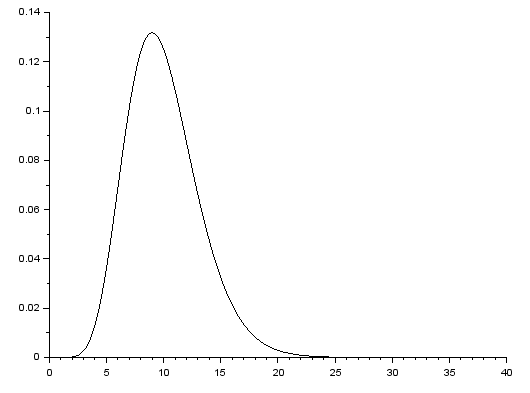
\includegraphics[width=1\linewidth]{fonction_dispersion}}
\end{figure}
\end{minipage}

We consider that the individual created is really born if it is born in the following area (\textbf{intra spécific competition}) :
\begin{equation*}
 C_{x,Z} = \{  z \in \R^2 ~ tq  ~~\forall y \in V(Z)\setminus \{x \}, ~~ |y-z|>distanceCompetition \}  
\end{equation*} 

\end{frame}





\begin{frame}{Mortality}

\begin{itemize}
\item Hypothesis: the mortality rate is independent of the position $x$ of an individual. \bigbreak
\item An individual living at time $t$ with a biomass $a(t)$ dies at the rate $m(a(t))$.
\bigbreak
\item The mortality $m$ is \textbf{a decreasing function of the biomass}: an individual with a low biomass, either because it has just been created or because it has undergone mowing, will have a higher rate of mortality.% ie taux de mortalité aux individus ayant un trait de biomasse faible.
\end{itemize}
\end{frame}





\subsubsection*{Evolution of the biomass:}

\begin{frame}{Evolution of the biomass}

The rhizome biomass associated with a crown evolves (in the absence of a mowing or mortality event) according to the following equation:
\begin{equation}
\label{VonBert}
\frac{da(t)}{dt}= L  ( K - a(t) ) 
\end{equation}

where $L$ is the low biomass growth rate and $K$ is the asymptotic biomass.

\bigbreak 

We are able to solve explicitly Equation \eqref{VonBert}.

We denote by $A_b$ the flow: $ t \rightarrow A_b(t,t_0,a_0)$ associated with the ordinary differential equation \eqref{VonBert}.
\end{frame}



%%%%%%%%%%%%%%%%%%%%%%%%%%%%%%%%%%%%%

\begin{frame}{Mowing}
Effects of mowing on rhizome development are poorly known.
\begin{itemize}
\item Hypothesis: reduction of underground biomass, rhizome resources used for growth of aerial parts \textcolor{red}{\cite{gerber2010evaluating}, \cite{rouifed2011contrasting}}
\item No influence of the distribution of the mowing dates, only the mowing number matters \textcolor{red}{\cite{seiger1997mechanical}}
\item Modeling choice: after a mowing, the underground biomass is directly impacted and becomes $a.F (a)$, where $F(a) \in [0,1]$. It is assumed that the effect of mowing is more important for low biomasses $ \Rightarrow F$ \textbf{increasing}.
\end{itemize}

\begin{equation*}
\forall a \in \R_+, ~F(a) = 1- exp(-mowingParameter  * a)
\end{equation*} 

\end{frame}



%%%%%%%%%%%%%%%%%%%%%%%%%%%%%%%%%%%%%%%
%  MPP , après l'EDS
%%%%%%%%%%%%%%%%%%%%%%%%%%%%%%%%%%%%


\begin{frame}{Poisson Point Measure} 
\addtocounter{framenumber}{-1}
An application $M : \Omega \times E \rightarrow \R_+ $ is a \textbf{random measure} if 
\begin{itemize}
\item $\omega  \rightarrow M(\omega,A)$ is a random variable for each $ A \in E$
\item $ A \rightarrow M(\omega,A)$ is a measure on $(E, \Ecal)$ for each $\omega \in \Omega$. We denote $M(A)$ this random variable.
\end{itemize} 
  
 % On peut alors voir $M$ comme une collection de variables aléatoires $ M(A), A \in E$.  On note  $M_\omega$ la mesure  $ A \rightarrow M(\omega,A)$.
 
The term "random measure" means that $M$ is a random variable that associate a measure $M_\omega$ to each event $ \omega \in \Omega$. 
 
\begin{Def}
Let $(E, \Ecal)$ be a measurable set and $ \nu$ be a measure on $(E, \Ecal)$.
A random measure $N$ on $(E, \Ecal)$ is a Poisson random measure with intensity $\nu$
if :

- for each $A \in E$, the random $N(A)$ has a Poisson law with parameter $ \nu(A)$.

-  for each $A_1,\ldots,A_n \in \Ecal$ disjoints, random variables  $(N(A_1), \ldots, N(A_n))$ are independents, for all  $n \geq 2$.
\end{Def}

\end{frame}
	%\backupend


%%%%%%%%%%%%%%%%%%%%%%%%%%%%%%%%%%%%%%%
%  EDS
%%%%%%%%%%%%%%%%%%%%%%%%%%%%%%%%%%%%
%\subsection*{Stochastic Differential Equation}
\begin{frame}{Stochastic Differential Equation}
\begin{align*}
\label{equation_sto} 
 Z_t & =  \sum_{i=1}^{N_0} \delta_{( X_i(Z_0) , A_b(t,0,A_i(Z_0) )} \\
 & +  \int_0^t \int_{\N^*} \int_{\R_+} \int_{\R^2}  1_{ \{  i \leq  N_{s-}  \} } \delta _{( X_i(Z_s)+z , A_b(t,s, a_0 ) ) } \\ 
& \times   1_{ \{  \theta \leq b(X_i(Z_s), Z_s ) \} }   1_{ \{ X_i(Z_s) + z ~ \in ~ C_{X_i(Z_s),Z_s} \} } \times M_1(ds,di,d\theta,dz) \\ 
& +  \int_0^t \int_{[0,1]^{N^*}}  ~ \sum_{i=1}^{N_{s^-}}  1_{ y_i \leq proportionMowing } ~\\
&( \delta_{( X_i(Z_s) , A_b(t,s,A_i(Z_{s^-}).F(A_i(Z_{s^-}) ) ))} -  \delta_{( X_i(Z_s) , A_b(t,s,A_i(Z_s)) )} )   M_2(ds,dy)  \\
&- \int_0^t \int_{\N^*} \int_{\R_+}  1_{ \{  i \leq  N_{s-}   \} }   1_{ \{  \theta \leq m( A_i(Z_s) ) \} }  \delta _{( X_i(Z_s) , A_b(t,s,A_i(Z_s) ) } M_3(ds,di,d\theta). 
\end{align*}

\small{$M_1(ds,di,d\theta,dz)$ is a Poisson point measure on $E_1:= \R_+ \times \N^* \times \R_+ \times  \R^2 $  with intensity $ \nu_1 = ds \otimes n(di)  \otimes d\theta \otimes  D(dz) $. }
\end{frame}




%%%%%%%%%%%%%%%%%%%%%%%%%%%%%%%%%%%%%%%
%  Large population limit 
%%%%%%%%%%%%%%%%%%%%%%%%%%%%%%%%%%%%
\begin{frame}{Large population limit}



\textbf{Objective:} Study of a renormalisation of the Stochastic Differential Equation solution $(Z^n)_{n \in \N}$ associated with the dynamics. 

\begin{itemize}
\item Simplification of the SDE: withdrawal the mowing term.

\item Initial population size of order $n$, no modification of the interaction between individuals. 
\end{itemize}

\smallbreak
\textbf{Result:} law convergence of the sequence of renormalised processes toward a process solution of an integro-differential equation :

\begin{flalign*}
 \langle \xi_t , f_t \rangle =  \langle \xi_0 , f_0 \rangle  +  
\int_0^t  \int_{\chi} \big[  v(a) \nabla_a f_s (x,a) + \frac{df_s}{ds}(x,a)  \\
  +\int_{\R^2} f_s(x+z,a_0)b(x,\xi_s ).h(x,z,\xi_s )d(dz)  -   f_s(x,a)  m(a) ) \big]  \xi_s (dx,da) ds. &&
\end{flalign*}

% Ainsi, en grande population, on pourra remplacer l'étude de l'équation différentielle stochastique par l'étude de cette nouvelle équation. 

\smallbreak
The techniques used for this result are those developed in \cite{tran2006modeles}.



\end{frame}




%%%%%%%%%%%%%%%%%%%%%%%%%%%%%%%%%%%%%%%%%%%%
%%  Loi des sorties : Cas moins sympa : quand extinction
%%%%%%%%%%%%%%%%%%%%%%%%%%%%%%%%%%%%%%%%%%%%
	%\backupbegin
\begin{frame}{Law of the output, with extinction}
\begin{figure}[H] 
\center{\includegraphics[width=0.6\linewidth]{"new picture pour aussois"/"tobbit extinction"}}
\caption{\footnotesize Empirical Cumulative Distribution Function of a Gausssian law with empirical mean and variance of the final area, for an initial population size = 1500, $\tau = 10$,  $proportionMowing = 0.9$, et $T=14$. There are 21 extinctions (over 50 simulations).}
\end{figure}
\end{frame}
	%\backupend


%%%%%%%%%%%%%%%%%%%%%%%%%%%%%%%%%%%%%%%
%  Method to assess general formulas
%%%%%%%%%%%%%%%%%%%%%%%%%%%%%%%%%%%%

\begin{frame}{Method to assess formulas}

Sobol sampling %(that maximizes discrepancy of the sequence, i.e. the space is evenly covered) 
of 5000 points with $ \tau \in [0 ; 15.0]$, $T \in  [0 ; 20]$,  and $initialPopSize \in [100 ; 1500]$. 

\bigbreak

\renewcommand{\arraystretch}{1.8}
\begin{tabular}{|l|l|l|l|}
	\hline
       		&  Mean Area   & Mean Size   \\  
   	\hline
    Regression tool &     \textit{lm}     &     \textit{nls}    \\
	\hline    
    Correlation &  $>0.99$  &  $>0.99$  \\
    \hline	    
    Residual standard error	& 2.23  &   26.12   \\
	\hline    
	\multirow{2}{*}{95 \% confident interval}  &  $c \in [ -0.0342 ; -0.0336]$  & $a \in [ 0. 90 ; 0.94 ]$   \\
 	\cline{2-3} 
	&  $ d \in [0.0960 ; 0.0998]$	  & $b \in [20.46 ; 20.77]$ \\ 
	\hline
\end{tabular}
\end{frame}











%%%%%%%%%%%%%%%%%%%%%%%%%%%%%%%%%%%%%%%%%%
%%%%  BIBLIO  
%%%%%%%%%%%%%%%%%%%%%%%%%%%%%%%%%%%%%%%%%%
\bibliographystyle{apalike}

%\begin{frame}{}
%\bibliography{biblio_rapport}
%%\printbibliography
%%\printbibliography[keyword=tran]
%\end{frame}

%	\backupbegin
\begin{frame}[allowframebreaks]
\tiny\bibliographystyle{apalike}
\tiny\bibliography{biblio_rapport}
\end{frame}
	\backupend

%\begin{frame}[allowframebreaks]
%        \frametitle{References}
%        \bibliographystyle{amsalpha}
%		\bibliography{biblio_rapport}
%\end{frame}


\end{document}
